\chapter{Lecture 19: Abstract Base Classes, Factory Method, Template Method, NVI, Maps}
\begin{center}
\textit{March 15, 2018}
\end{center}

\section{Partial and Mixed Assignment: The Fix}
\begin{lstlisting}[style=cpp]
Text a{...}, b{...};
Book *pa{&a};
Book *pb{&b};
*pa = *pb;      // partial assignment
\end{lstlisting}
Making \code{operator=} virtual forces
\code{Text \&Text::operator=(const Book \&)}, which allows mixed assignment.

\paragraph{Solution.} Restructure the hierarchy: make the base class abstract,
give it a \emph{protected} assignment operator, and make each kind of book
(including plain ``normal'' books) a concrete subclass.

\begin{figure}[H]
\centering
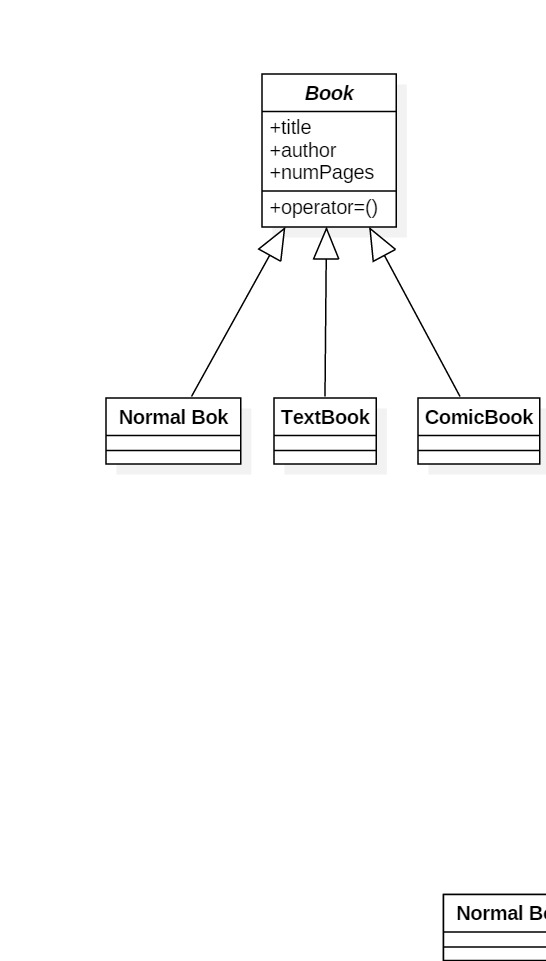
\includegraphics[width=0.5\textwidth, trim=0 480 0 60, clip]{figures/book-uml.jpg}
\caption{Abstract \code{Book} (italic name) with concrete subclasses
\code{NormalBook}, \code{TextBook} and \code{ComicBook}.}
\end{figure}

\begin{lstlisting}[style=cpp]
class AbstractBook {
    std::string title, author;
    int numPages;
  protected:
    AbstractBook &operator=(const AbstractBook &other);  // subclasses only
  public:
    AbstractBook(...);
    virtual ~AbstractBook() = 0;     // abstract; still needs a body
};
AbstractBook::~AbstractBook() {}

class NormalBook : public AbstractBook {
  public:
    NormalBook &operator=(const NormalBook &other) {
        AbstractBook::operator=(other);
        return *this;
    }
};

class Text : public AbstractBook {
    std::string topic;
  public:
    Text &operator=(const Text &other) {
        AbstractBook::operator=(other);
        topic = other.topic;
        return *this;
    }
};
// Comic is similar
\end{lstlisting}
\begin{lstlisting}[style=cpp]
AbstractBook *pa1{&a};
AbstractBook *pb1{&b};
*pa1 = *pb1;    // won't compile: AbstractBook::operator= is protected
a = b;          // fine: Text::operator=, full assignment
\end{lstlisting}
Partial and mixed assignment through base pointers are now both impossible,
while assignment between objects of the same concrete type still works.

\begin{important}[Advice]
In a class hierarchy, make superclasses abstract. (Non-leaf classes should be
abstract.)
\end{important}

\section{The Factory Method Pattern}
Problem: write a video game with two kinds of enemies, turtles and bullets. The
system randomly sends turtles and bullets, but bullets are more frequent in
harder levels. We never know exactly which enemy comes next, so we can't call
the Turtle or Bullet ctor directly; and the decision policy depends on the level.

\begin{lstlisting}[style=cpp]
class Level {
  public:
    virtual Enemy *createEnemy() = 0;   // the factory method
    virtual ~Level() {}
};

class Normal : public Level {
  public:
    Enemy *createEnemy() override {
        // more turtles (they are easier to kill)
    }
};

class Castle : public Level {
  public:
    Enemy *createEnemy() override {
        // more bullets
    }
};

Player *p = ...;
Level *l = new Normal;
Enemy *e = nullptr;
while (p->notDead()) {
    e = l->createEnemy();     // generate an enemy: the level decides which
    // attack the player
}
\end{lstlisting}

Also called the \textbf{Virtual Constructor pattern}: \code{createEnemy} acts
like a constructor whose concrete class is chosen at run time. A related idea:
make a class's constructors private/protected and provide methods that create
objects for the client. We have seen this already: \code{List::addToFront}
creates Nodes; \code{List::begin}/\code{List::end} create Iterators.

\section{The Template Method Pattern}
We want to allow subclasses to override \emph{some} aspects of the superclass's
behaviour, while other aspects must remain the same.

Example: red turtles and green turtles. Drawing a turtle means drawing a head,
a shell and feet; only the shell differs.
\begin{lstlisting}[style=cpp]
class Turtle {
  public:
    void draw() {           // the template method: not virtual
        drawHead();
        drawShell();
        drawFeet();
    }
    virtual ~Turtle() {}
  private:
    void drawHead() { ... }
    void drawFeet() { ... }
    virtual void drawShell() = 0;   // the customizable step
};

class RedTurtle : public Turtle {
    void drawShell() override { /* draw a red shell */ }
};

class GreenTurtle : public Turtle {
    void drawShell() override { /* draw a green shell */ }
};
\end{lstlisting}
Subclasses can't change the overall drawing algorithm (\code{draw} is not
virtual) but they can (must) supply the shell. Note that a subclass may override
a private virtual method, even though it cannot call it.

\section{The Non-Virtual Interface (NVI) Idiom}
Think about what a \textbf{public virtual} method means:
\begin{itemize}
  \item \textbf{public}: the class promises clients a certain, pre-defined
        behaviour (an interface, with pre/post-conditions);
  \item \textbf{virtual}: an invitation to subclasses to change that behaviour
        to anything they like.
\end{itemize}
These pull in opposite directions: we cannot guarantee the behaviour if
subclasses can replace it.

\begin{important}[NVI idiom]
\begin{itemize}
  \item All public methods should be non-virtual (except the destructor).
  \item All virtual methods should be private (or protected, if subclasses need
        to call the base version).
\end{itemize}
\end{important}

\begin{lstlisting}[style=cpp]
class DigitalMedia {         // not following NVI
  public:
    virtual void play() = 0;
    virtual ~DigitalMedia() {}
};

class DigitalMedia {         // using NVI
  public:
    void play() {
        checkCopyright();    // the base class keeps control:
        doPlay();            // e.g. copyright check before, stats after
    }
    virtual ~DigitalMedia() {}
  private:
    void checkCopyright();
    virtual void doPlay() = 0;
};
\end{lstlisting}
With NVI, the base class can later add code before/after every call (logging,
checks) without changing any subclass. It costs nothing (\code{play} can be
inlined), so the advice is to always use it. It generalizes the Template Method
pattern: every virtual method is wrapped in a non-virtual template method.

\section{The STL \code{map}}
A \code{map} is a generalization of an array where the key (index) and the value
can be of any type (the key type must support \code{operator<}, since maps are
kept sorted --- typically as balanced binary search trees). It is a template
class parameterized on two types.
\begin{lstlisting}[style=cpp]
#include <map>
...
map<string, int> m;
m["abc"] = 1;
m["def"] = 4;
cout << m["abc"] << endl;   // prints 1
cout << m["ghi"] << endl;   // prints 0: if the key is absent, operator[]
                            // default-constructs a value and inserts it!

if (m.count("def")) { ... } // lookup without inserting:
                            // 0 if no such key, 1 if found
m.erase("abc");
\end{lstlisting}
Another STL class, \code{multimap}, allows several values per key --- look at it
on your own time.

Surprise, surprise: an iterator is predefined.
\begin{lstlisting}[style=cpp]
for (auto &p : m) {
    // p has type std::pair<const string, int> (a struct in the STL)
    cout << p.first << " " << p.second << endl;   // fields, not methods
}
\end{lstlisting}
Iteration happens in sorted key order.

\section{The Visitor Pattern: Double Dispatch}
The Visitor pattern is used for \textbf{double dispatch}: choosing which method to
call based on the run-time types of \emph{two} objects.

Example: enemies and weapons. The effect of striking depends on both the kind of
enemy and the kind of weapon.
\begin{quote}
\textit{``Enenemy --- that's not how you spell enemy.''} --- Nomair
\end{quote}
\begin{lstlisting}[style=cpp]
class Enemy {
  public:
    virtual void strike(Rock &) = 0;
    virtual void strike(Stick &) = 0;
};
\end{lstlisting}
This assumes we know the exact type of the weapon at compile time. Gameplay
doesn't look like that:
\begin{lstlisting}[style=cpp]
Enemy *e = l->createEnemy();
Weapon *w = p->chooseWeapon();
e->strike(*w);      // which strike? *w is only known to be a Weapon
\end{lstlisting}
C++ dynamically dispatches on the object a method is called on, but not on the
argument types (overloading is resolved at compile time).

The Visitor pattern is a clever combination of overriding and overloading:
\begin{lstlisting}[style=cpp]
class Enemy {
  public:
    virtual void strike(Weapon &w) = 0;
    virtual ~Enemy() {}
};

class Turtle : public Enemy {
  public:
    void strike(Weapon &w) override { w.useOn(*this); }  // *this is a Turtle
};
class Bullet : public Enemy {
  public:
    void strike(Weapon &w) override { w.useOn(*this); }  // *this is a Bullet
};

class Weapon {
  public:
    virtual void useOn(Turtle &t) = 0;
    virtual void useOn(Bullet &b) = 0;
    virtual ~Weapon() {}
};

class Stick : public Weapon {
  public:
    void useOn(Turtle &t) override { /* stick on turtle */ }
    void useOn(Bullet &b) override { /* stick on bullet */ }
};
class Rock : public Weapon {
  public:
    void useOn(Turtle &t) override { /* rock on turtle */ }
    void useOn(Bullet &b) override { /* rock on bullet */ }
};
\end{lstlisting}
The two \code{strike} bodies look identical, but putting them in \code{Enemy}
to reuse code would be wrong: the whole point is that inside \code{Turtle}, the
type of \code{*this} is known to be \code{Turtle}, which selects the right
overload of \code{useOn}.

\begin{lstlisting}[style=cpp]
Enemy *e = ...;   // suppose it is a Turtle
Weapon *w = ...;  // suppose it is a Stick
e->strike(*w);
\end{lstlisting}
\begin{enumerate}
  \item \code{strike} is virtual: \code{Turtle::strike} runs (dispatch on the
        enemy);
  \item it calls \code{w.useOn(*this)} with \code{*this} of static type
        \code{Turtle\&}: overload resolution picks \code{useOn(Turtle\&)};
  \item \code{useOn} is virtual: \code{Stick::useOn(Turtle\&)} runs (dispatch on
        the weapon).
\end{enumerate}
More uses of Visitor next lecture.

\section*{Summary}
\begin{itemize}
  \item Fix partial/mixed assignment with an abstract base class whose
        \code{operator=} is protected; make non-leaf classes abstract.
  \item Factory Method: a virtual method creates objects whose concrete type the
        subclass decides.
  \item Template Method: a non-virtual algorithm calls virtual steps.
  \item NVI: public methods non-virtual, virtual methods private.
  \item \code{map<K,V>}: \code{operator[]} inserts defaults; use \code{count} to
        test membership; iteration yields sorted \code{pair}s.
  \item Visitor: \code{strike} (override) + \code{useOn(*this)} (overload) gives
        double dispatch.
\end{itemize}
